\chapter{Diseño del sistema}
En esta sección se va a mostrar el diseño de la aplicación. Se detallará sobre el modelo de datos, aspectos de seguridad y diseño visual de la aplicación.

\subsection{Modelo de datos}
Para poder empezar con la implementación es de vital importancia definir cuáles son los datos que vamos a manipular en la aplicación, que entidades representan y como se relacionan estas entidades.

    \begin{figure}[H]
        \centering
        \includegraphics[width=0.9\linewidth]{images/diagramaLógicoV3.png}
        \caption{Modelo lógico de datos}
        \label{fig:diagramaER}
    \end{figure}

% Para facilitar la explicación de lo anterior mencionado nos referiremos a la figura \ref{fig:diagramaER}
\subsubsection{Usuario}
Un usuario representa a una persona que utiliza la aplicación. Cada usuario tiene un identificador único, un nombre, una dirección de correo electrónico, una contraseña, un nombre de usuario, una marca de tiempo de cuando se unió a la aplicación, y una ubicación preferida.

\subsubsection{Grupo}
Un grupo es una entidad que representa un conjunto de usuarios que se han unido para comunicarse y colaborar. Cada grupo tiene un identificador único, un nombre, una descripción, un límite de miembros, lugar y tipo de grupo. También el grupo mantiene la referencia al usuario dueño del grupo.

\subsubsection{Mensaje}
Un mensaje es una entidad que representa la comunicación entre usuarios dentro de un grupo.Cada mensaje mantiene una referencia al grupo y al usuario que lo envió, el contenido del mensaje, una marca de tiempo de cuando se envió. Cada mensaje también mantiene una lista con las referencias de los usuarios que han leído dicho mensaje.

\subsubsection{Membresía}
La membresía es una entidad intermedia que representa la relación entre los usuarios y los grupos. Es decir, denota que un usuario se ha unido a un grupo. Cada membresía tiene un identificador único, el identificador del usuario, el identificador del grupo, y una marca de tiempo de cuando el usuario se unió al grupo.

\subsubsection{Evento}
El entidad evento viene siempre asociada a un grupo, este describe el encuentro de grupo. Mantiene campos como título, descripción, marca de tiempo, fecha de celebración y un campo booleano que identifica la flexibilidad horaria.

\subsubsection{Asistencia}
La asistencia como su nombre indica, identifica la asistencia de un usuario a un evento. Tiene un identificador compuesto por dos claves foráneas, en este caso los identificadores de evento y usuario. Así como dos campos opcionales de tipo marca de tiempo que identifican la preferencia del tiempo de comienzo y final del evento en el caso en el que este último permita la flexibilidad horaria.

\begin{comment}
\subsection{Aspectos de Seguridad}
Es importante considerar aspectos de seguridad en el diseño de la aplicación. Por ejemplo, las contraseñas de los usuarios deben ser almacenadas de manera segura utilizando métodos de hash y sal. Además, debería haber autenticación y autorización adecuadas para asegurar que los usuarios solo puedan realizar acciones que les estén permitidas, como por ejemplo, un usuario solo puede eliminar un grupo si es el dueño de este.
\end{comment}

\subsection{Navegación y vistas}
\begin{figure}[H]
        \centering
        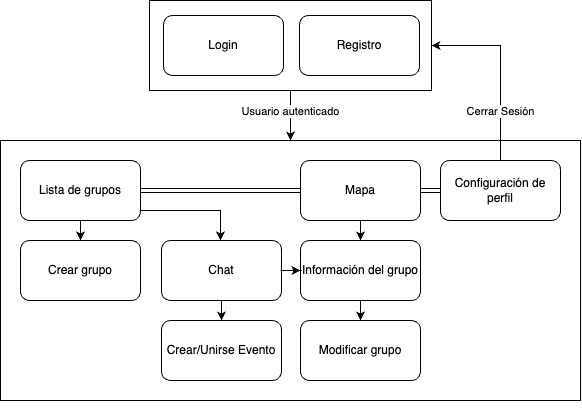
\includegraphics[width=1\linewidth]{images/diagramaNavegacion (1).png}
        \caption{Diagrama de navegación}
        \label{fig:diagramaER}
\end{figure}
La vistas de la aplicación se han encapsulado en distintos grupos:

\subsubsection{Login}
La pantalla \textit{Login} es el primer punto de entrada de nuestra aplicación, dónde el usuario puede tomar varias acciones: autenticarse, proceder al registro o restablecer contraseña.

\begin{figure}[H]
        \centering
        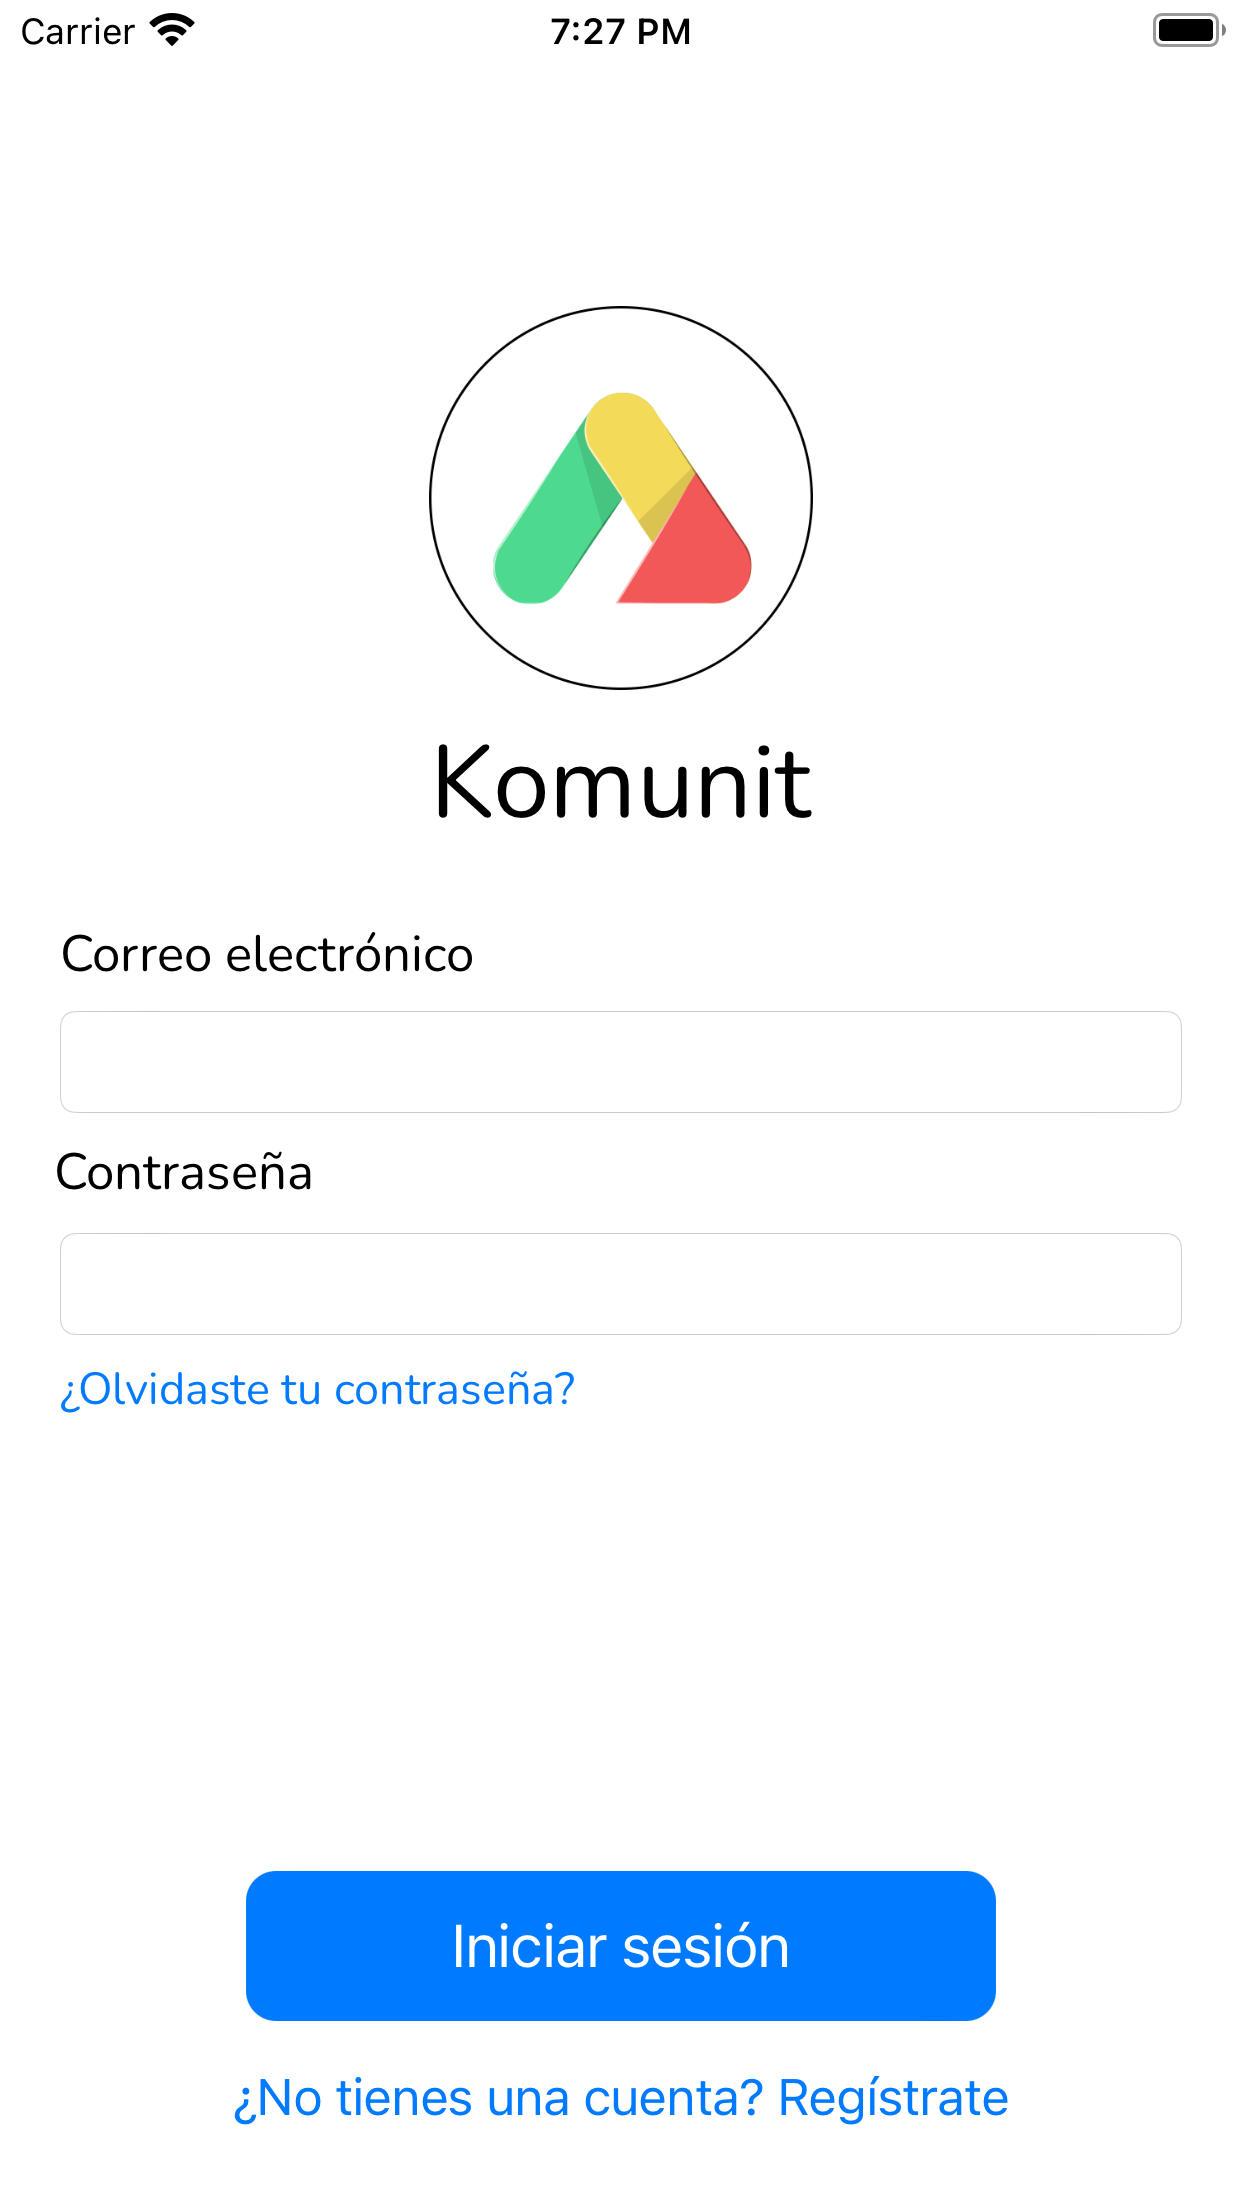
\includegraphics[cframe=black 2pt,width=0.3\linewidth]{images/manual/login.png}
        \caption{Inicio de sesión}
        \label{fig:Vista Inicio de Sesión}
\end{figure}

\subsubsection{Registro}
La vista de registro en donde el visitante procederá a rellenar sus datos tales como nombre, nombre de usuario, contraseña, entre otros.
\begin{figure}[H]
        \centering
        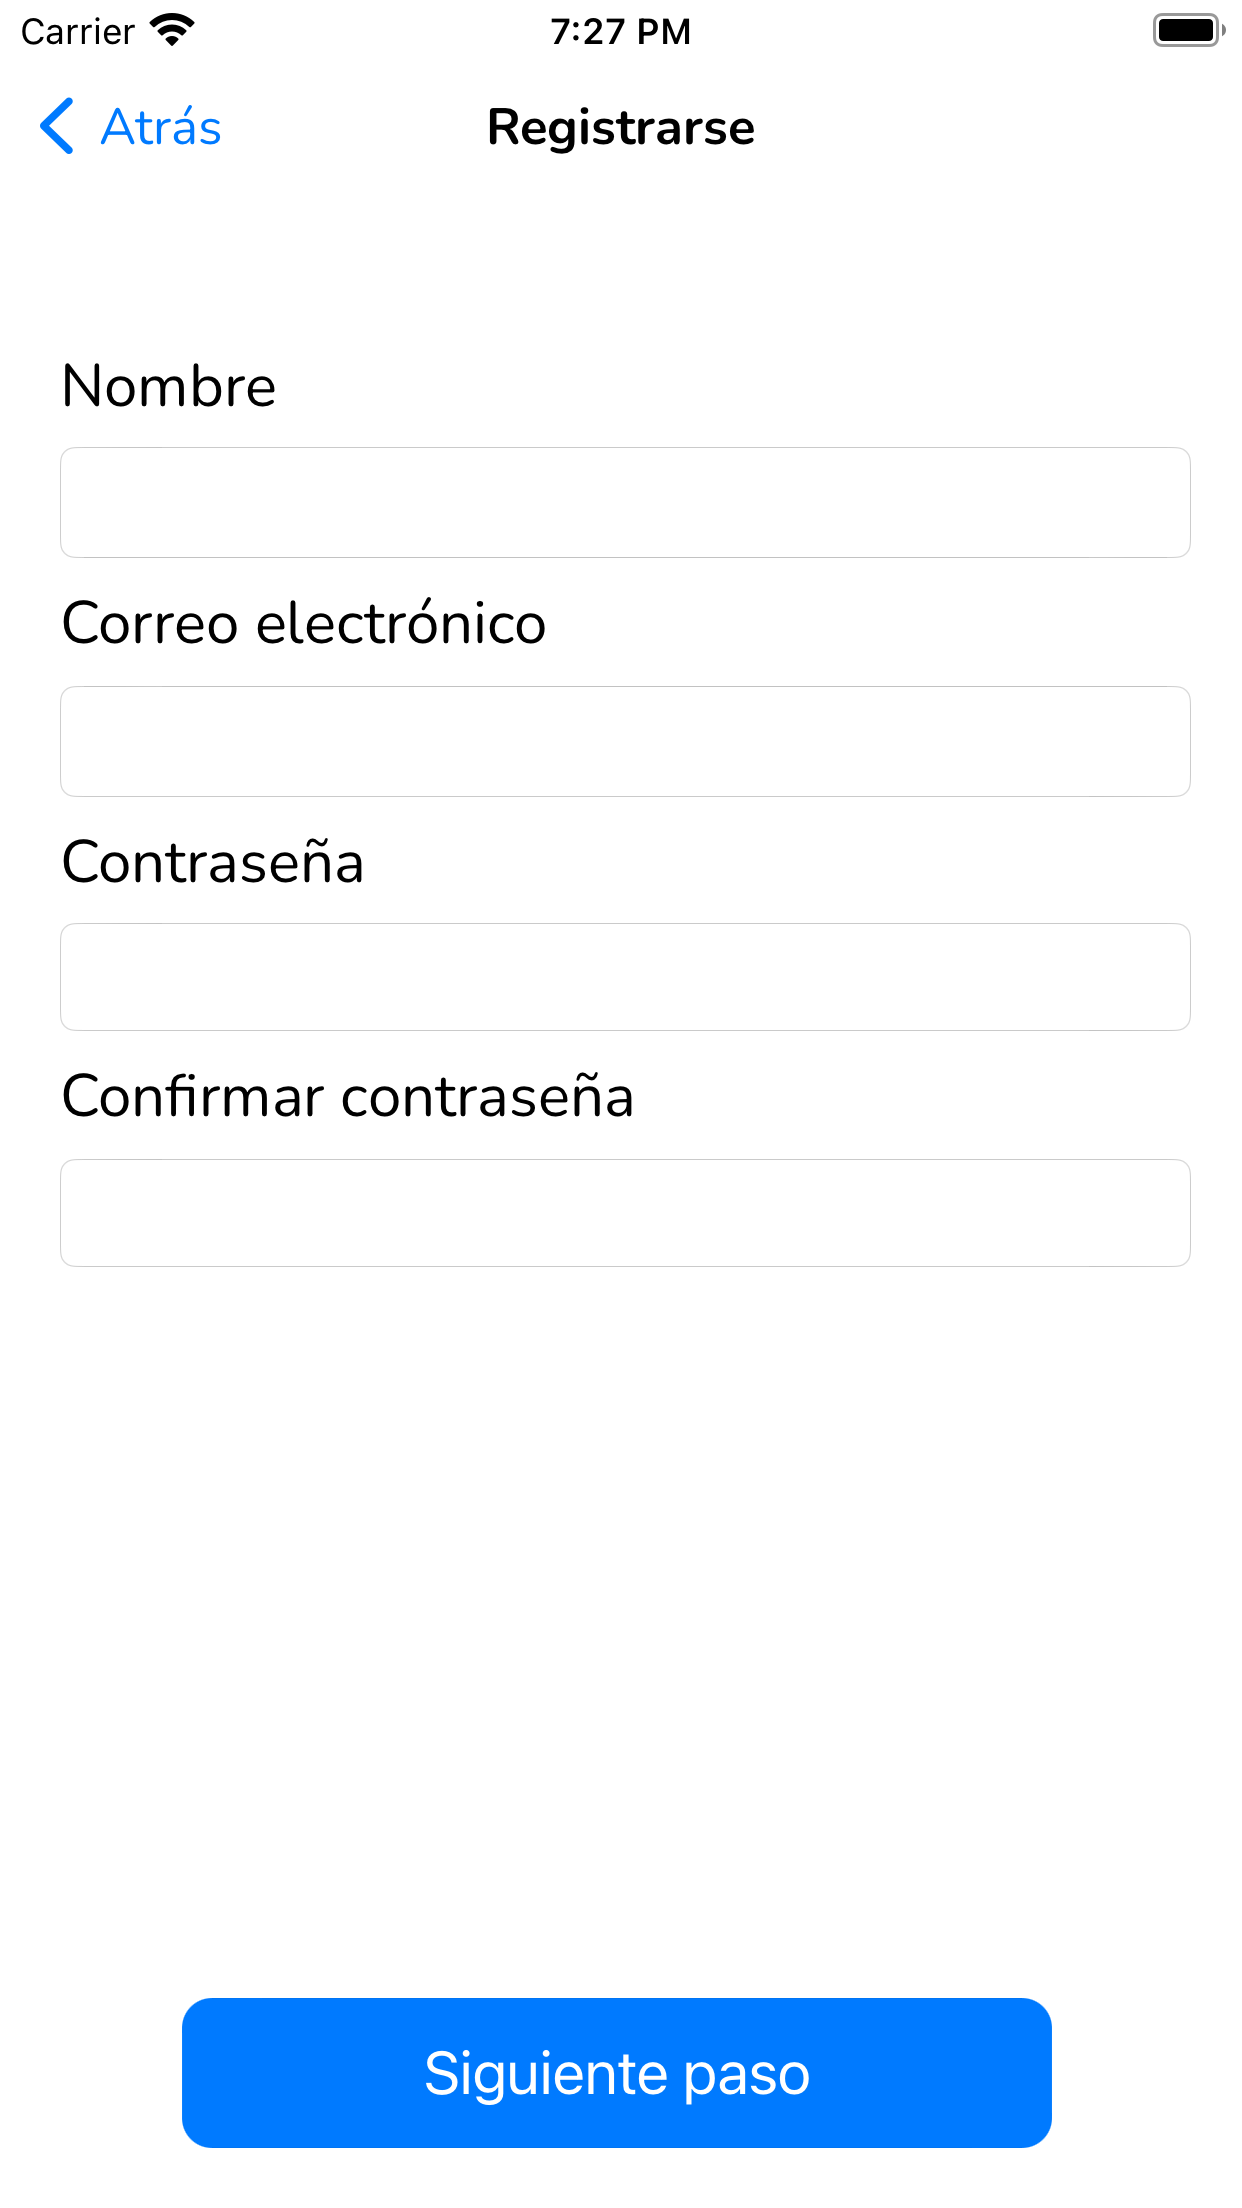
\includegraphics[cframe=black 2pt,width=0.3\linewidth]{images/manual/registro1.png}
        \caption{Registro de usuario}
        \label{fig:Vista Resgistro}
\end{figure}
\subsubsection{Confirmación de correo electrónico}
El usuario para dar por finalizado el registro deberá confirmar su correo electrónico.
\begin{figure}[H]
        \centering
        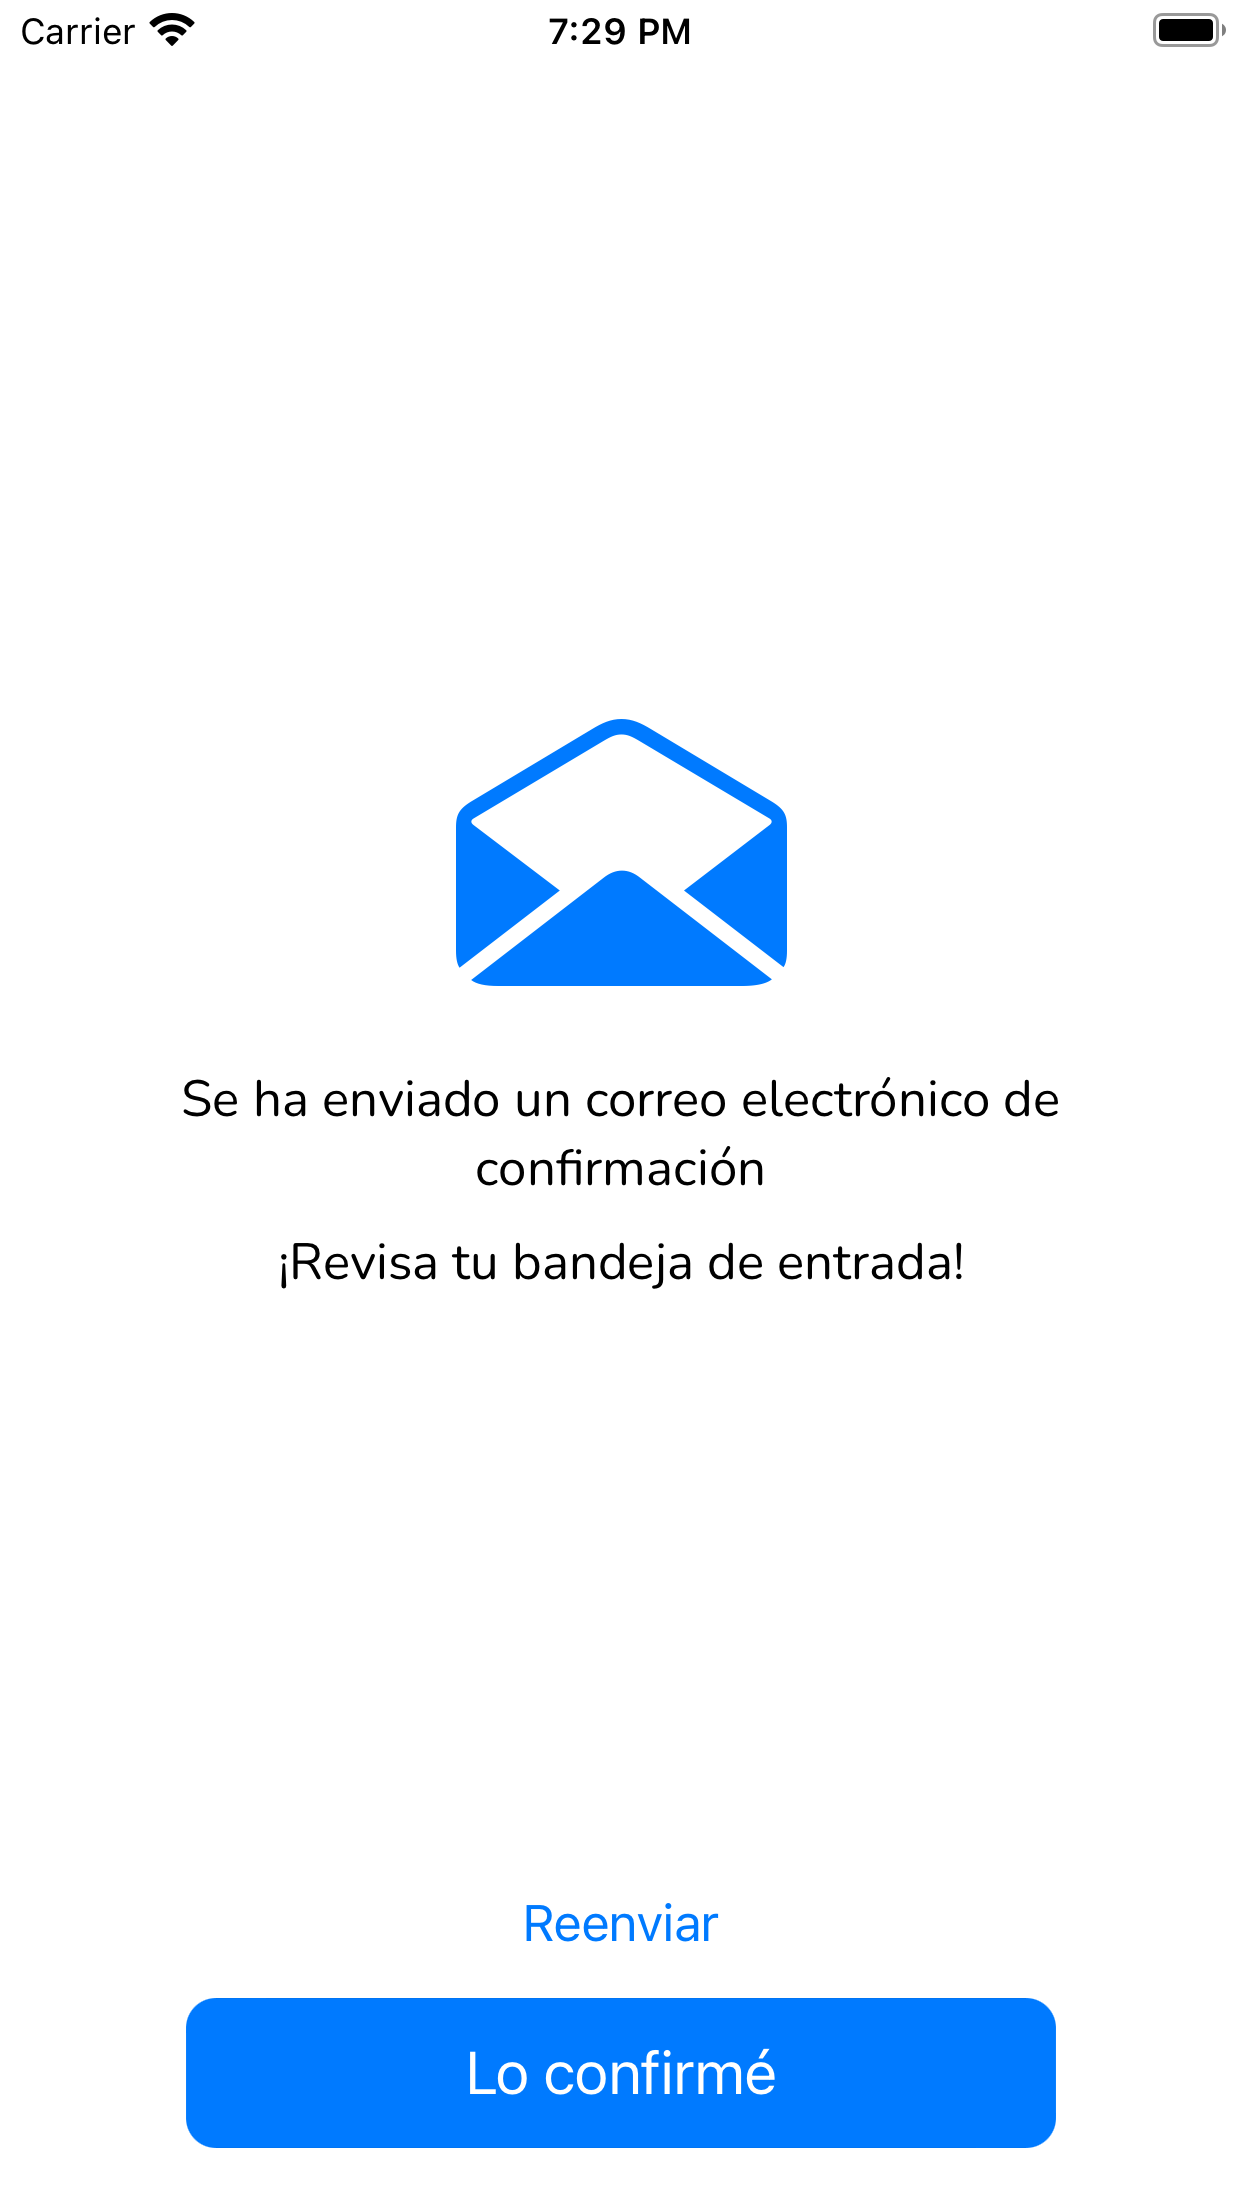
\includegraphics[cframe=black 2pt,width=0.3\linewidth]{images/manual/registroConfirmacion.png}
        \caption{Confirmación de correo}
        \label{fig:Vista Confirmación Correo Electrónico}
\end{figure}
\subsubsection{Mapa}
Es en el mapa donde el usuario podrá explorar de forma interactiva los distintos grupos alrededor suya.
\begin{figure}[H]
        \centering
        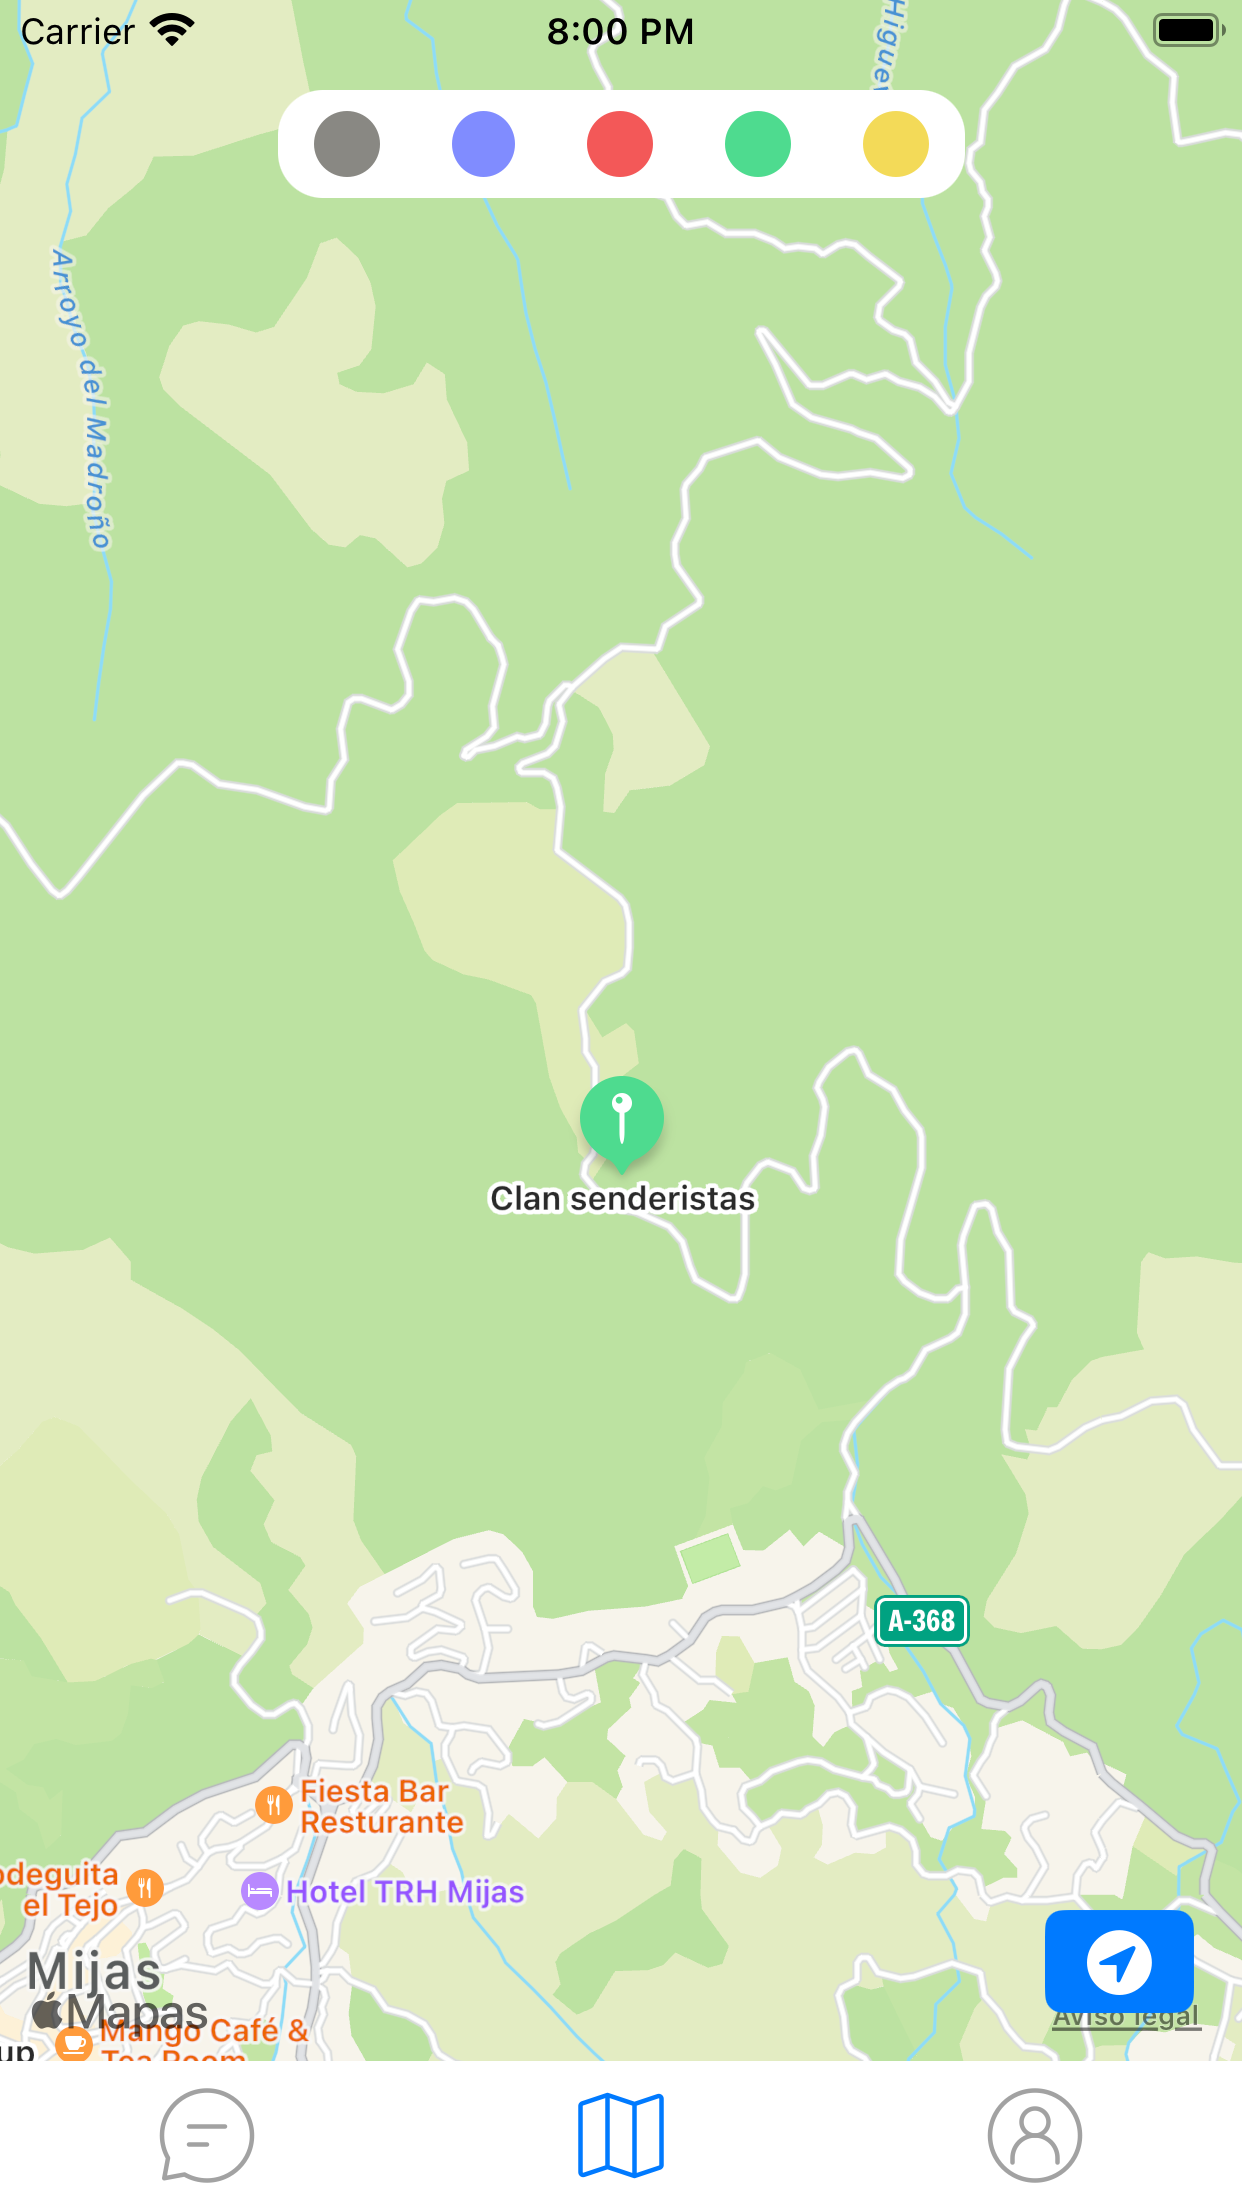
\includegraphics[cframe=black 2pt,width=0.3\linewidth]{images/manual/explorarGruposMapap.png}
        \caption{Vista mapa}
        \label{fig:Vista mapa}
\end{figure}
\subsubsection{Lista de grupos}
Vista con los distintos grupos a los que pertenece un usuario.
\begin{figure}[H]
        \centering
        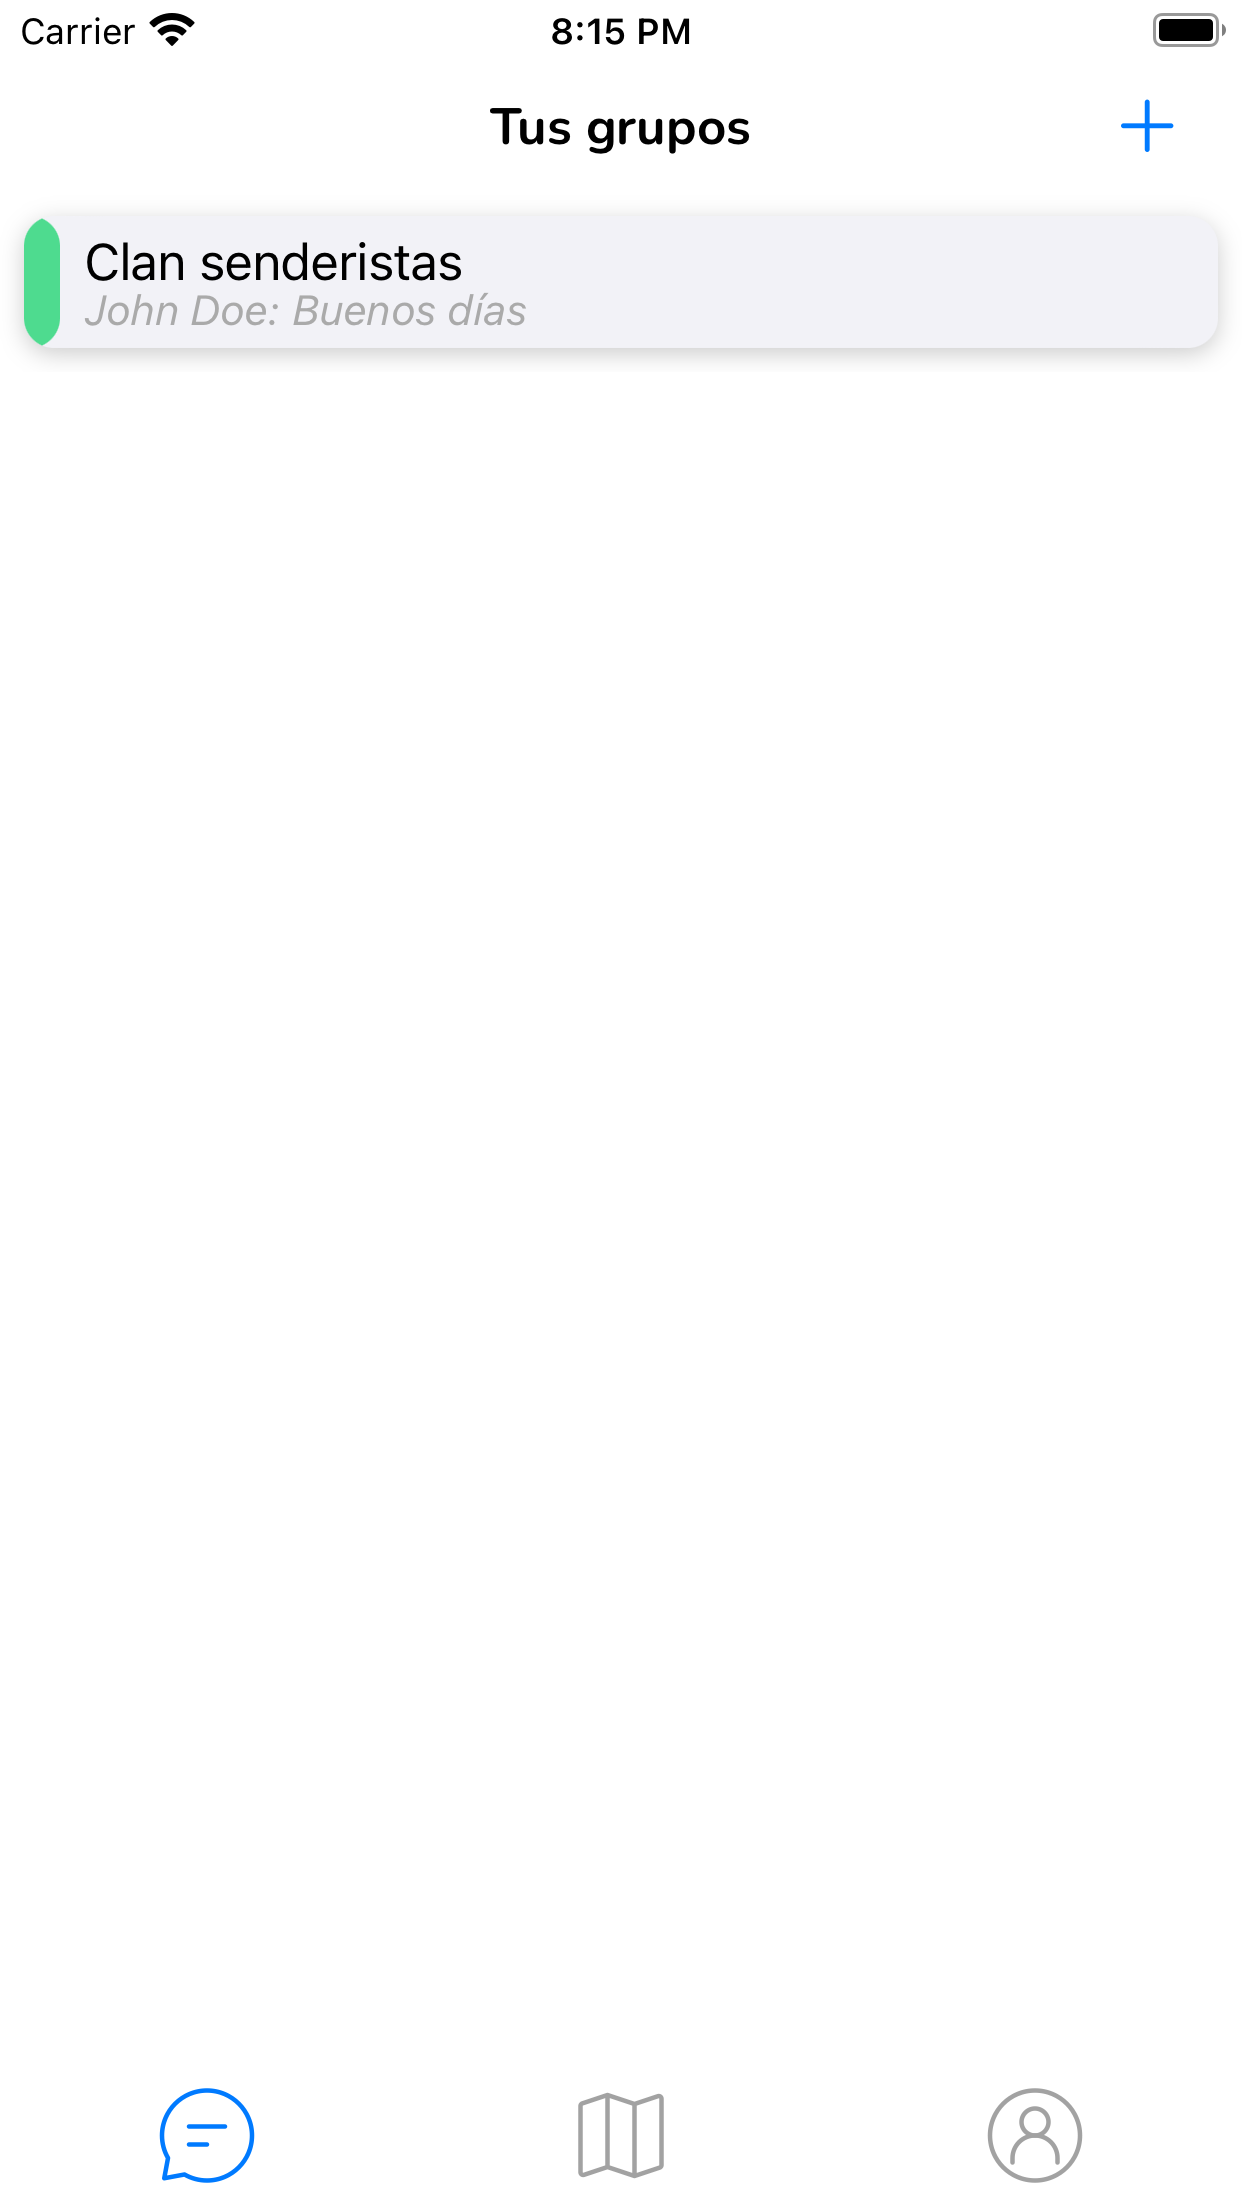
\includegraphics[cframe=black 2pt,width=0.3\linewidth]{images/manual/listadoGruposChats.png}
        \caption{Lista de grupos}
        \label{fig:Vista grupos}
\end{figure}
\subsubsection{Chat}
Vista del chat interno del grupo, donde el usuario puede ver los mensajes del resto de miembros y mandar en nombre propio.
\begin{figure}[H]
        \centering
        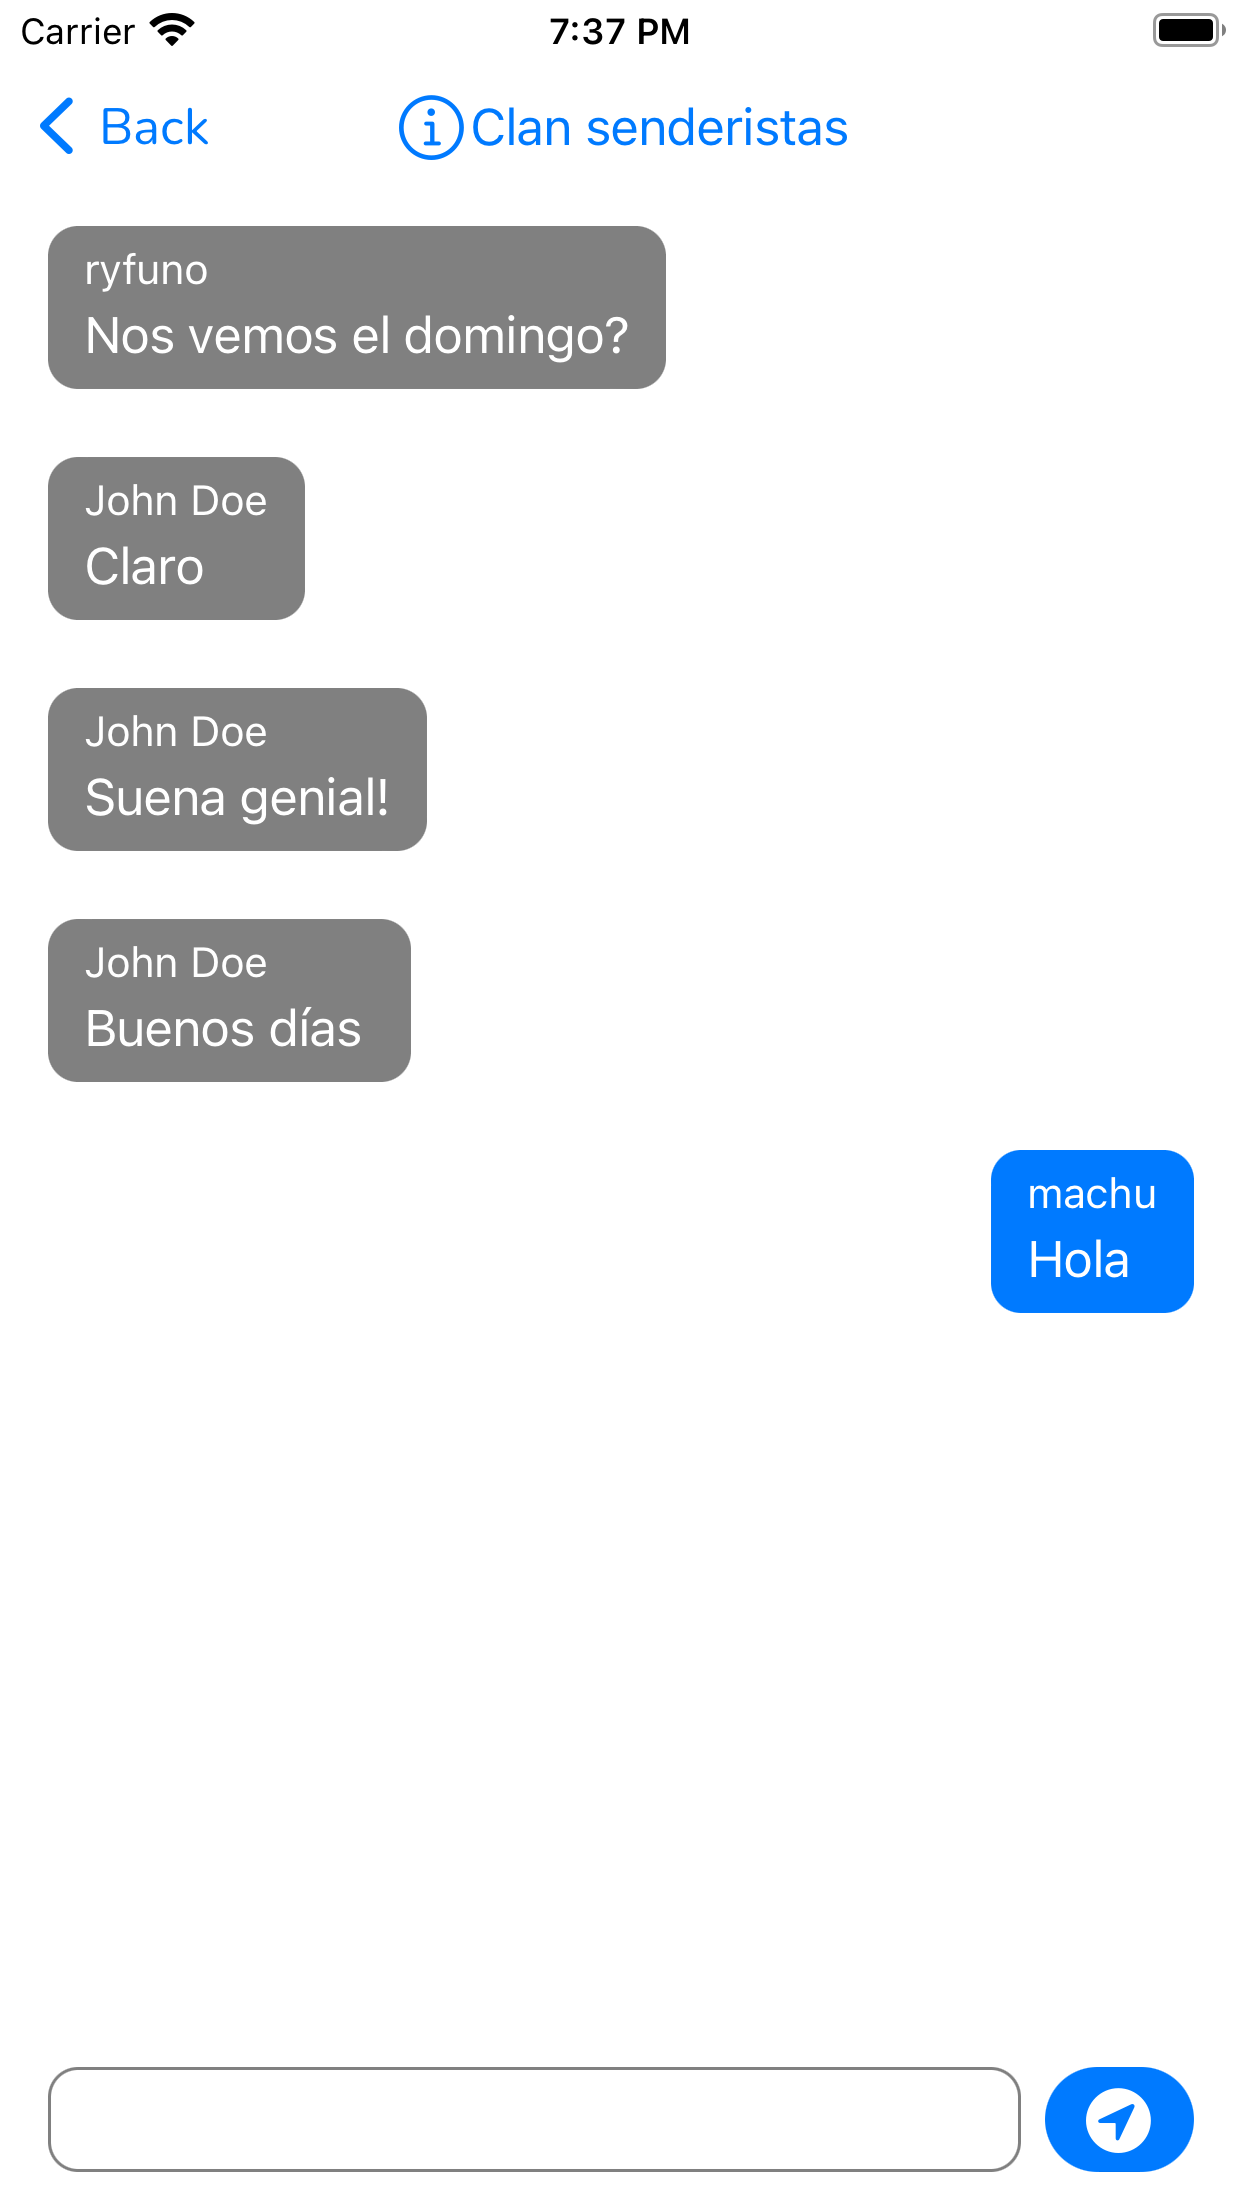
\includegraphics[cframe=black 2pt,width=0.3\linewidth]{images/manual/ejemploChat.png}
        \caption{Vista de chat de grupo}
        \label{fig:Vista chat grupo}
\end{figure}
\subsubsection{Detalle del grupo}
Vista con la información del grupo como título, descripción y tipo de grupo.
\begin{figure}[H]
        \centering
        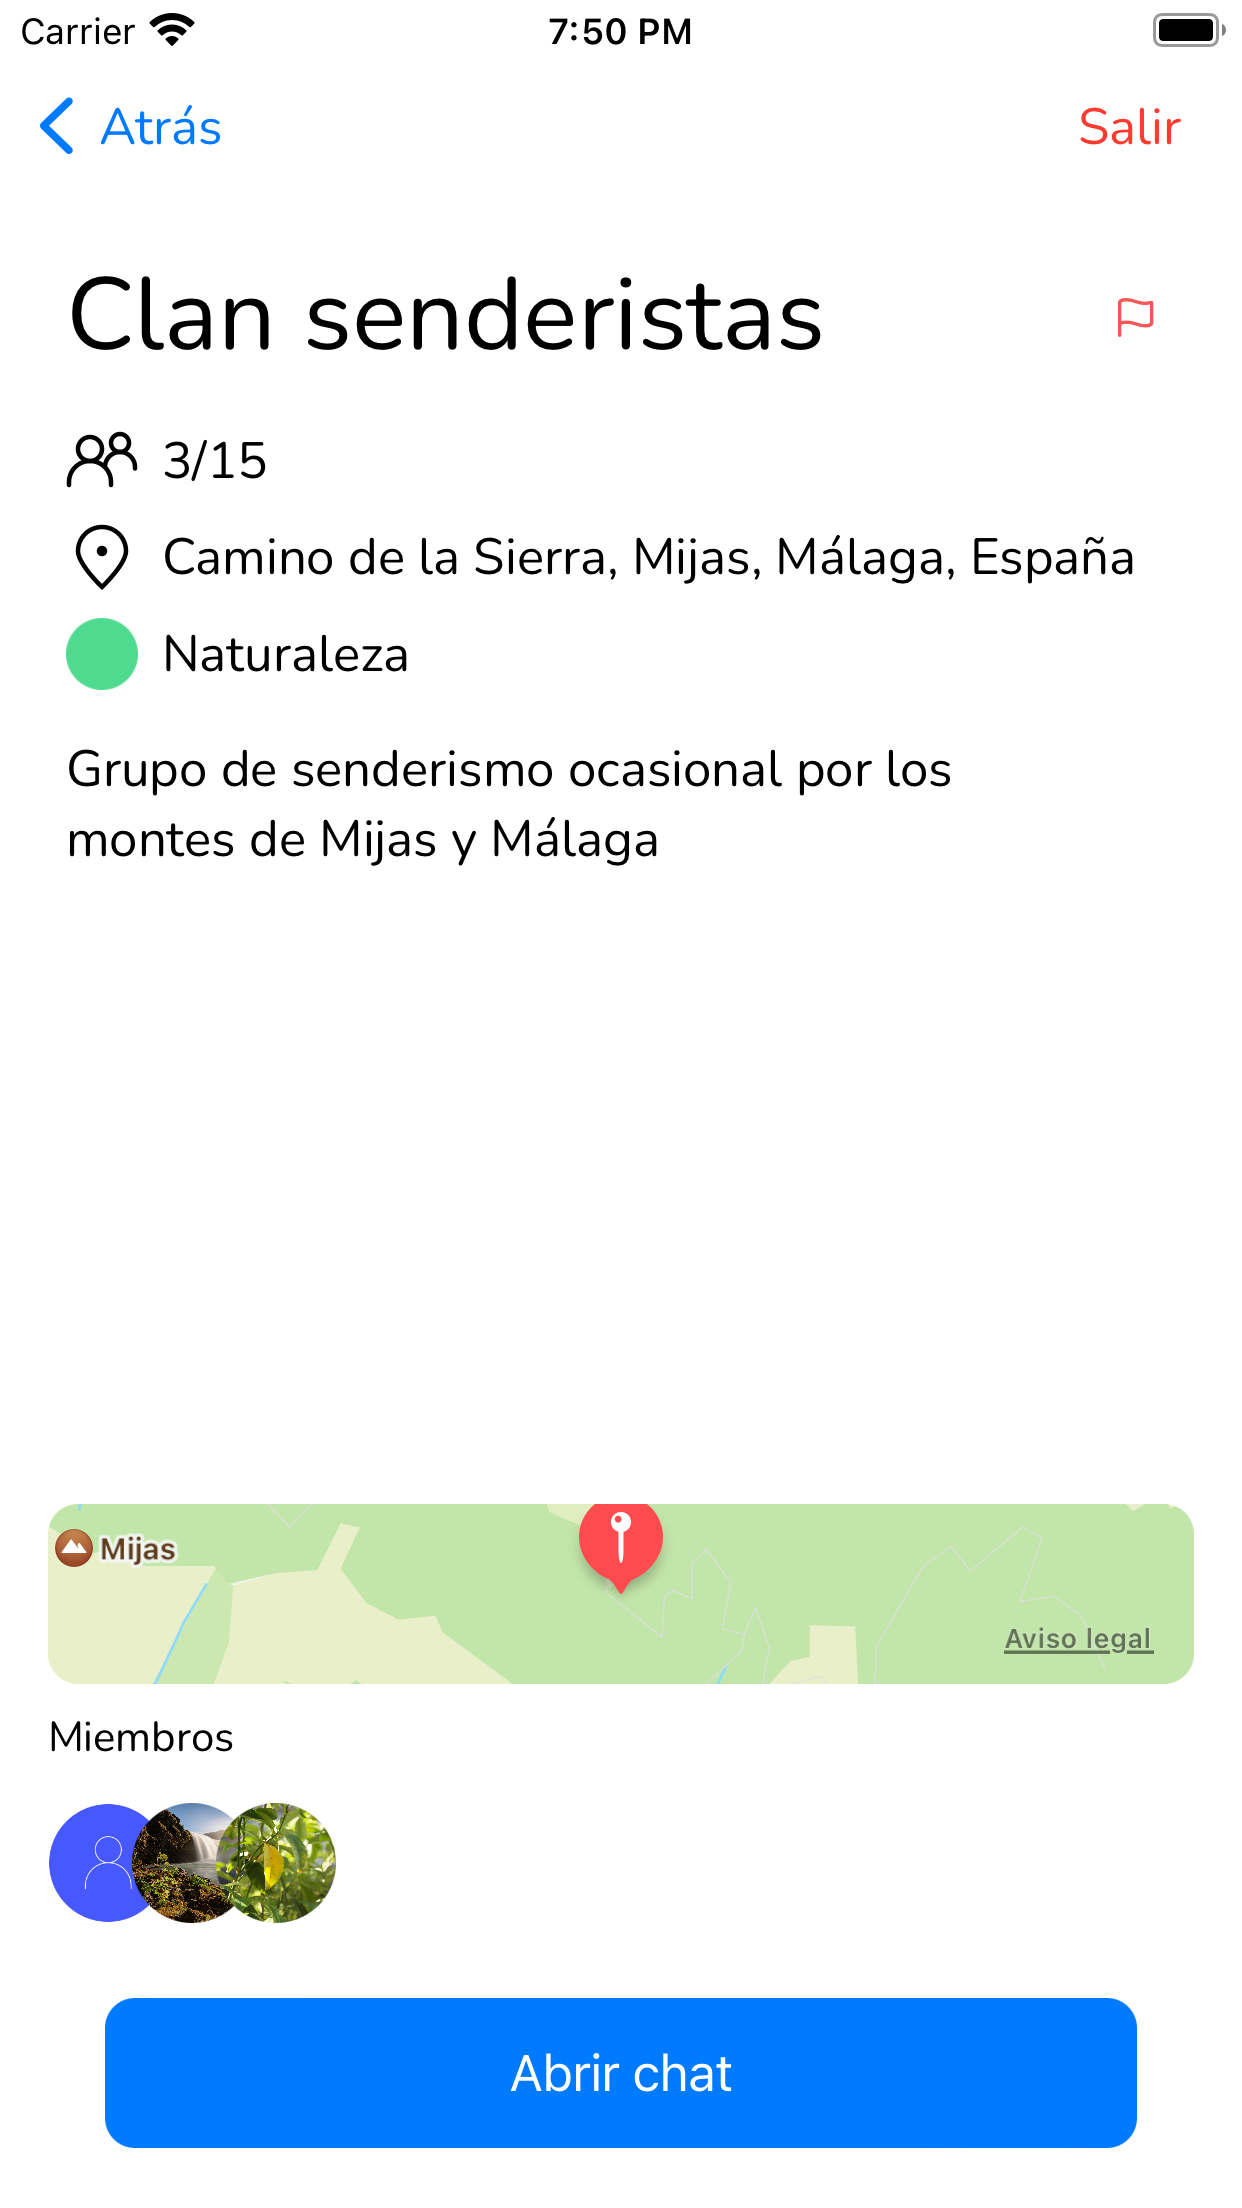
\includegraphics[cframe=black 2pt,width=0.3\linewidth]{images/manual/groupInfoAsMember.png}
        \caption{Vista detalle del grupo}
        \label{fig:Vista detalle del grupo}
\end{figure}
\subsubsection{Crear grupo}
Formulario de creación del grupo, el usuario deberá rellenar campos como título, localización, descripción, etc, para poder crear el grupo.
\begin{figure}[H]
        \centering
        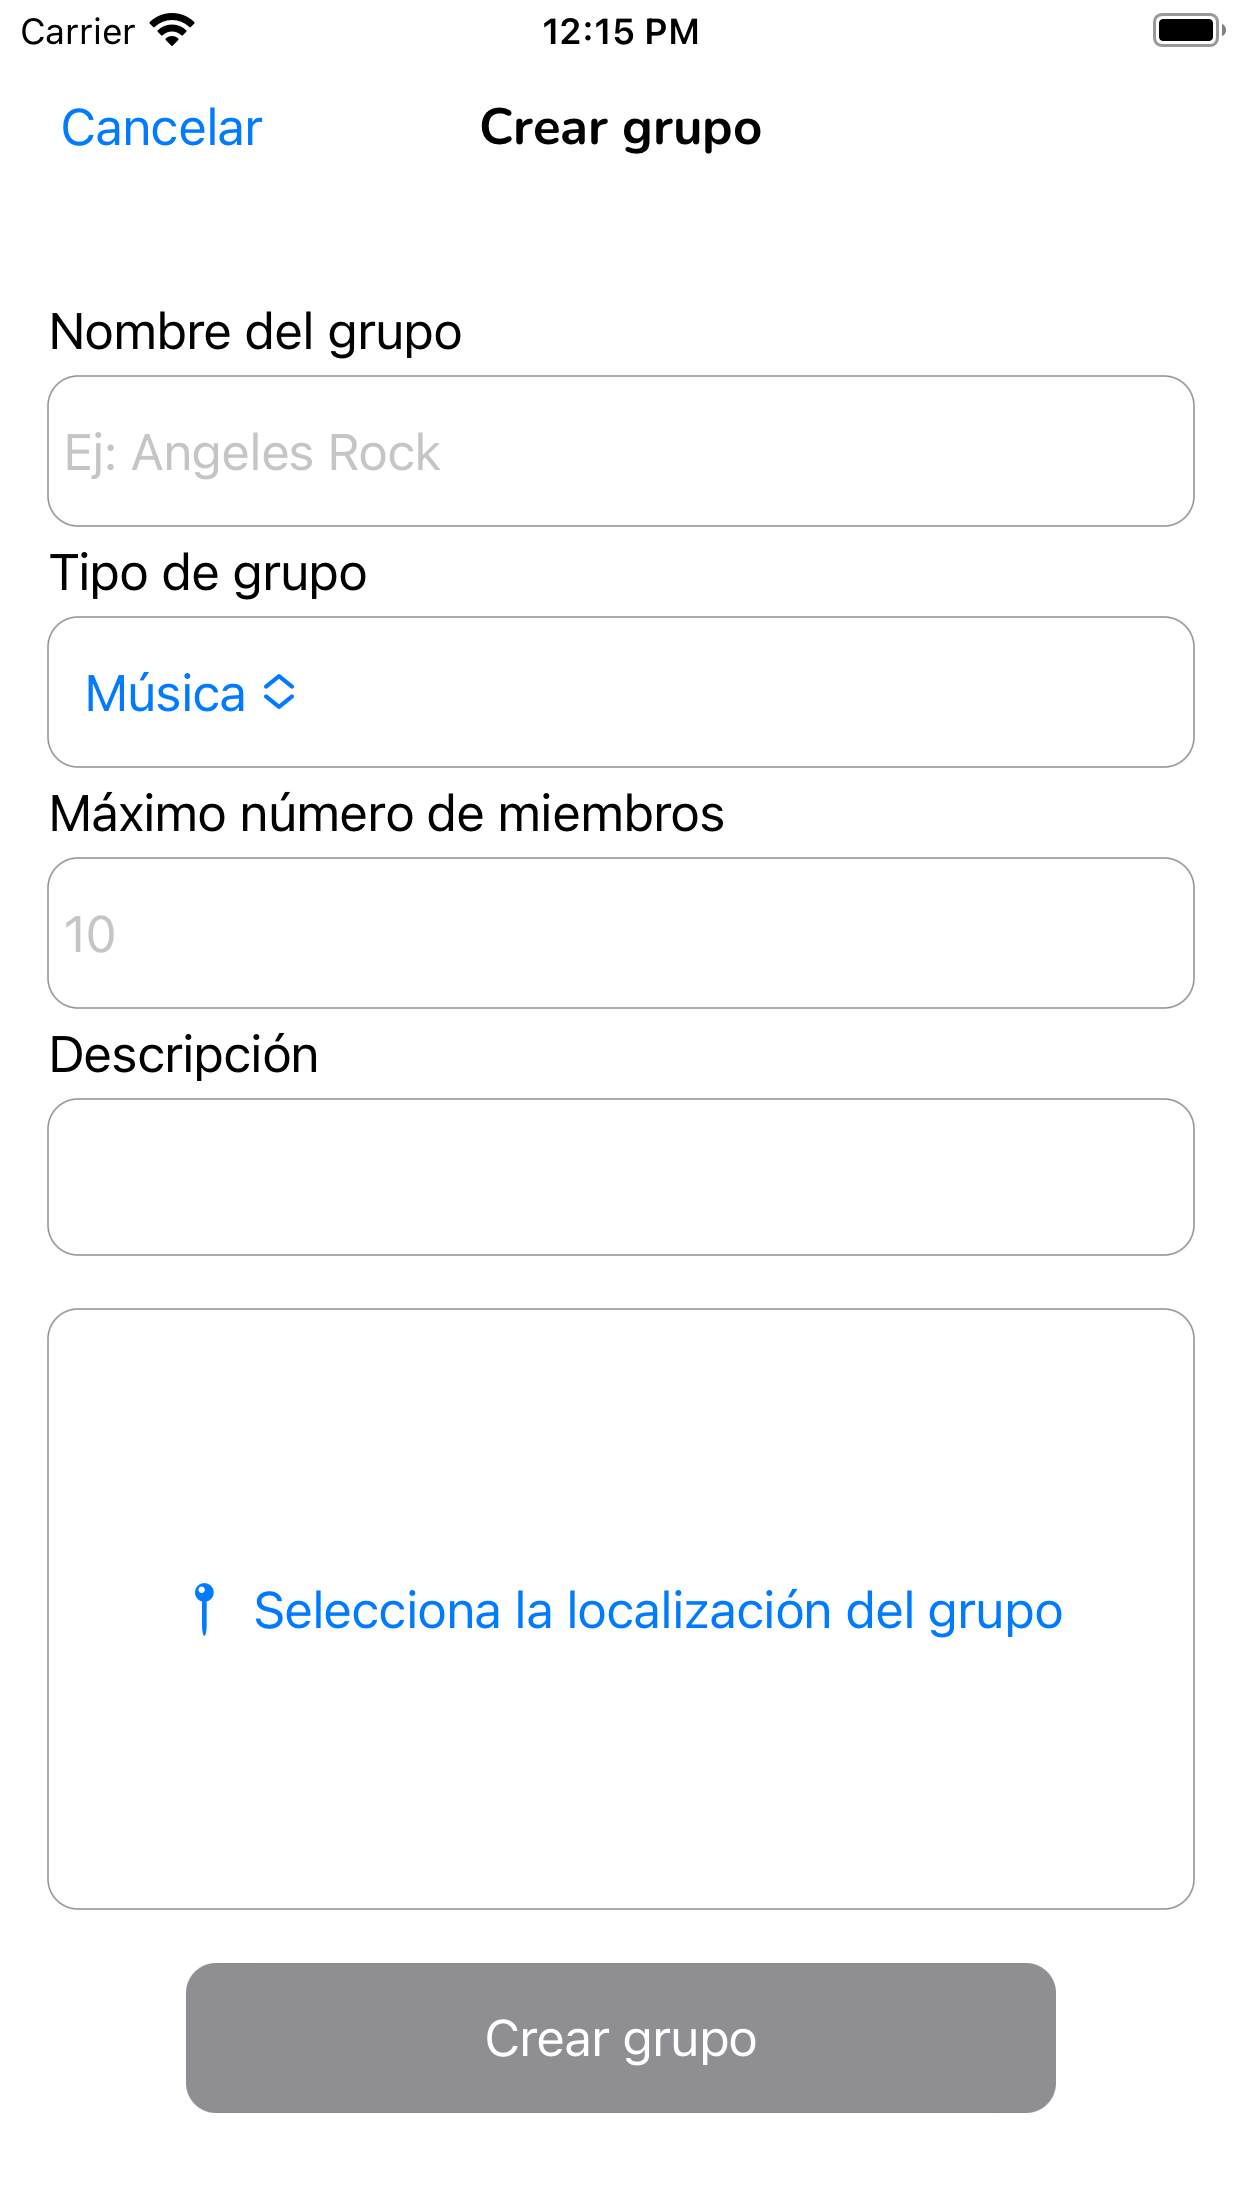
\includegraphics[cframe=black 2pt,width=0.3\linewidth]{images/manual/crearGrupo.png}
        \caption{Vista crear grupo}
        \label{fig:Vista Crear Grupo}
\end{figure}
\subsubsection{Perfil}
Vista con la información del usuario así como acciones adicionales .
\begin{figure}[H]
        \centering
        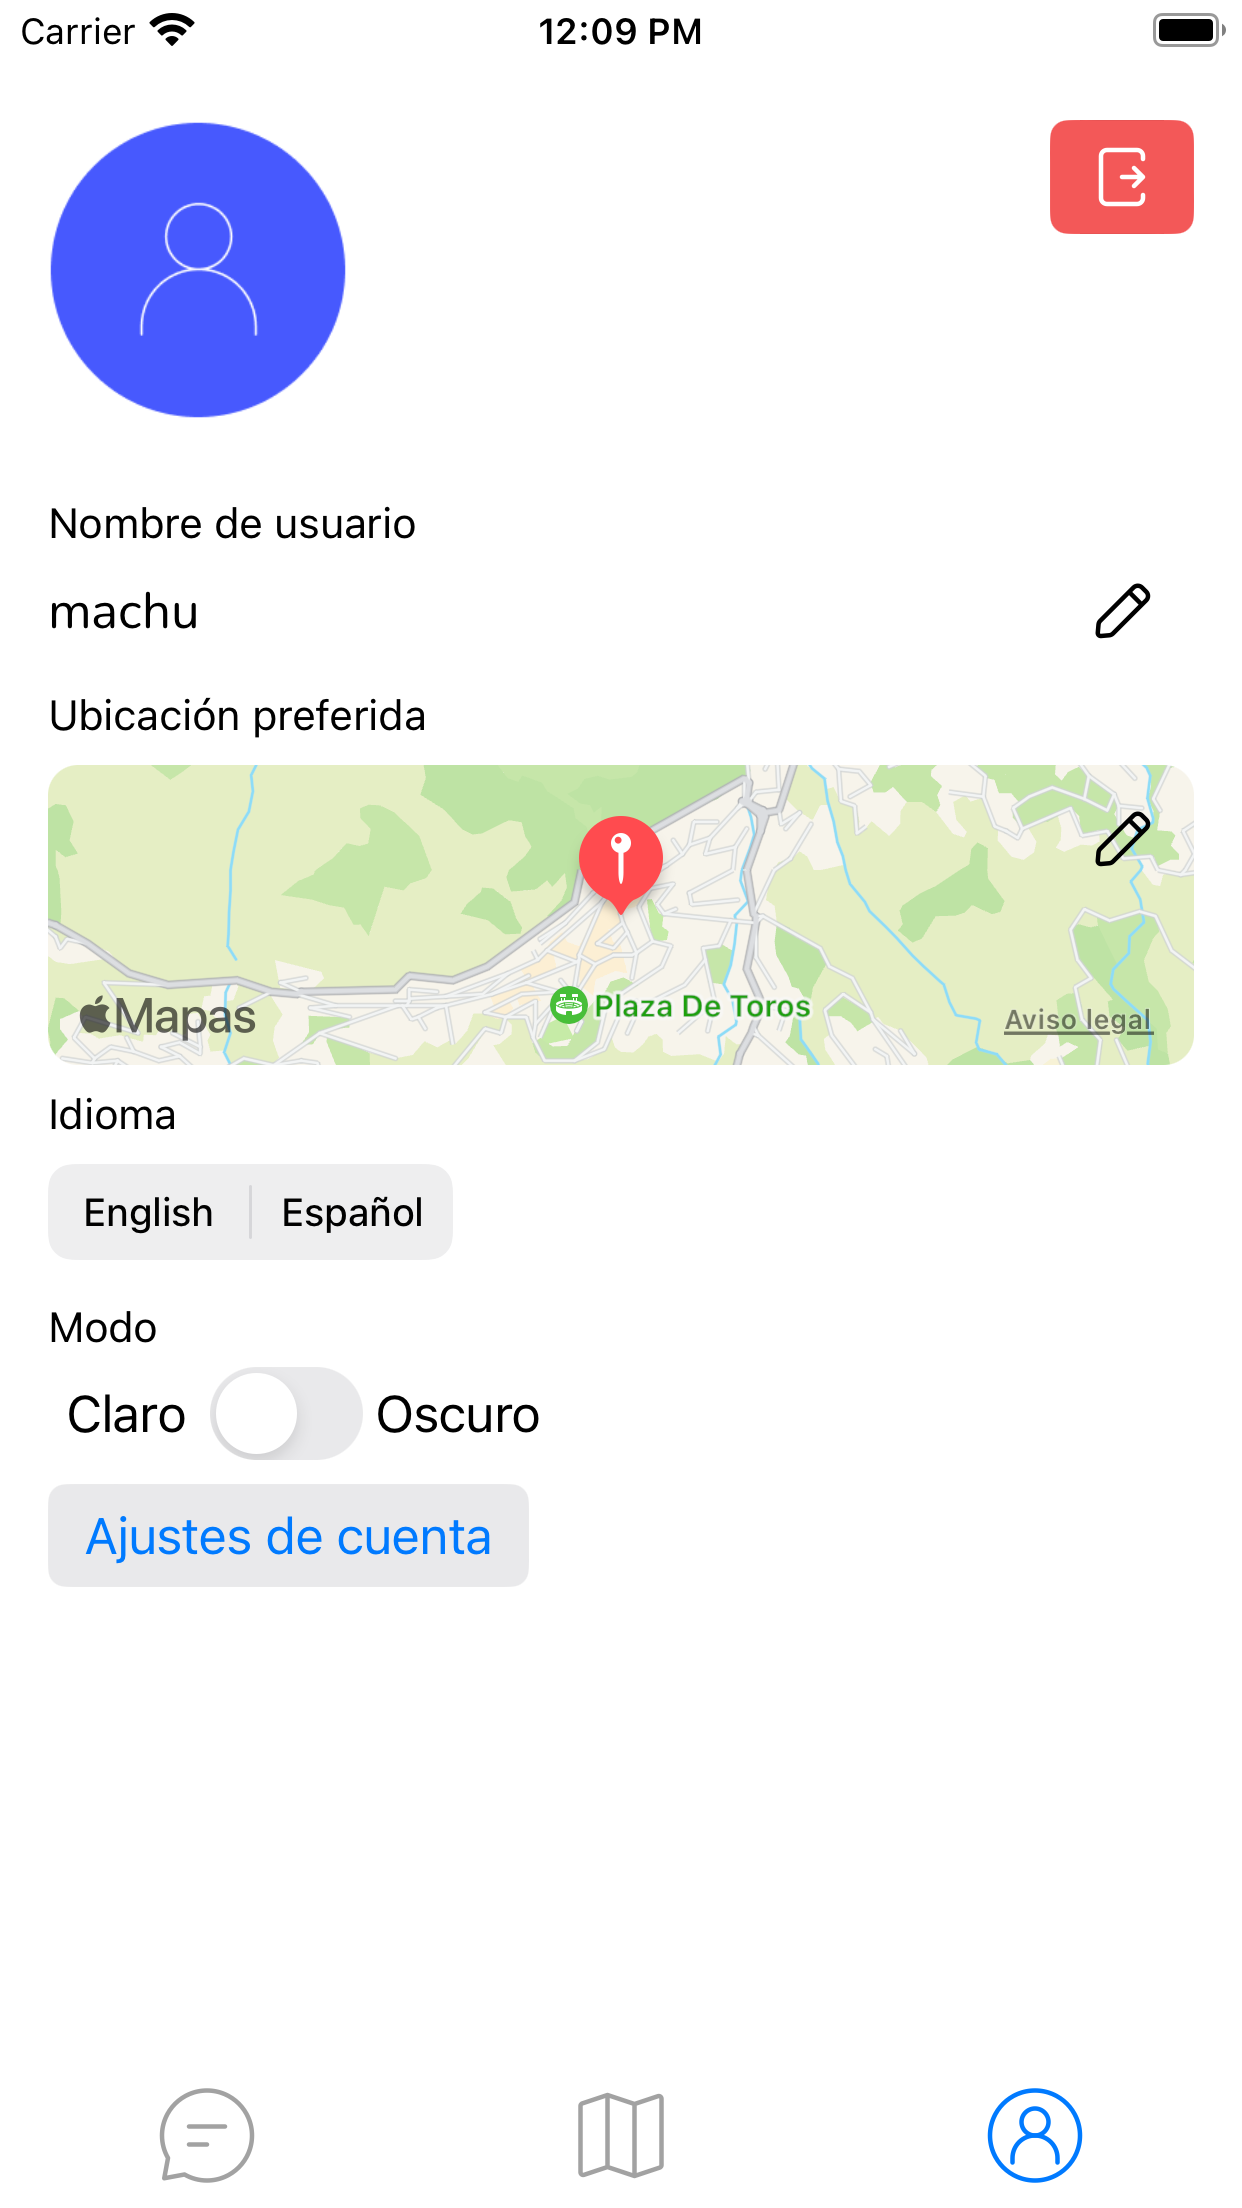
\includegraphics[cframe=black 2pt,width=0.3\linewidth]{images/manual/confPerfil.png}
        \caption{Vista Perfil}
        \label{fig:Vista Perfil}
\end{figure}

\subsection{Evento}
Vista desde la que se puede gestionar un evento o crear la asistencia a dicho evento.
\begin{figure}[H]
        \centering
        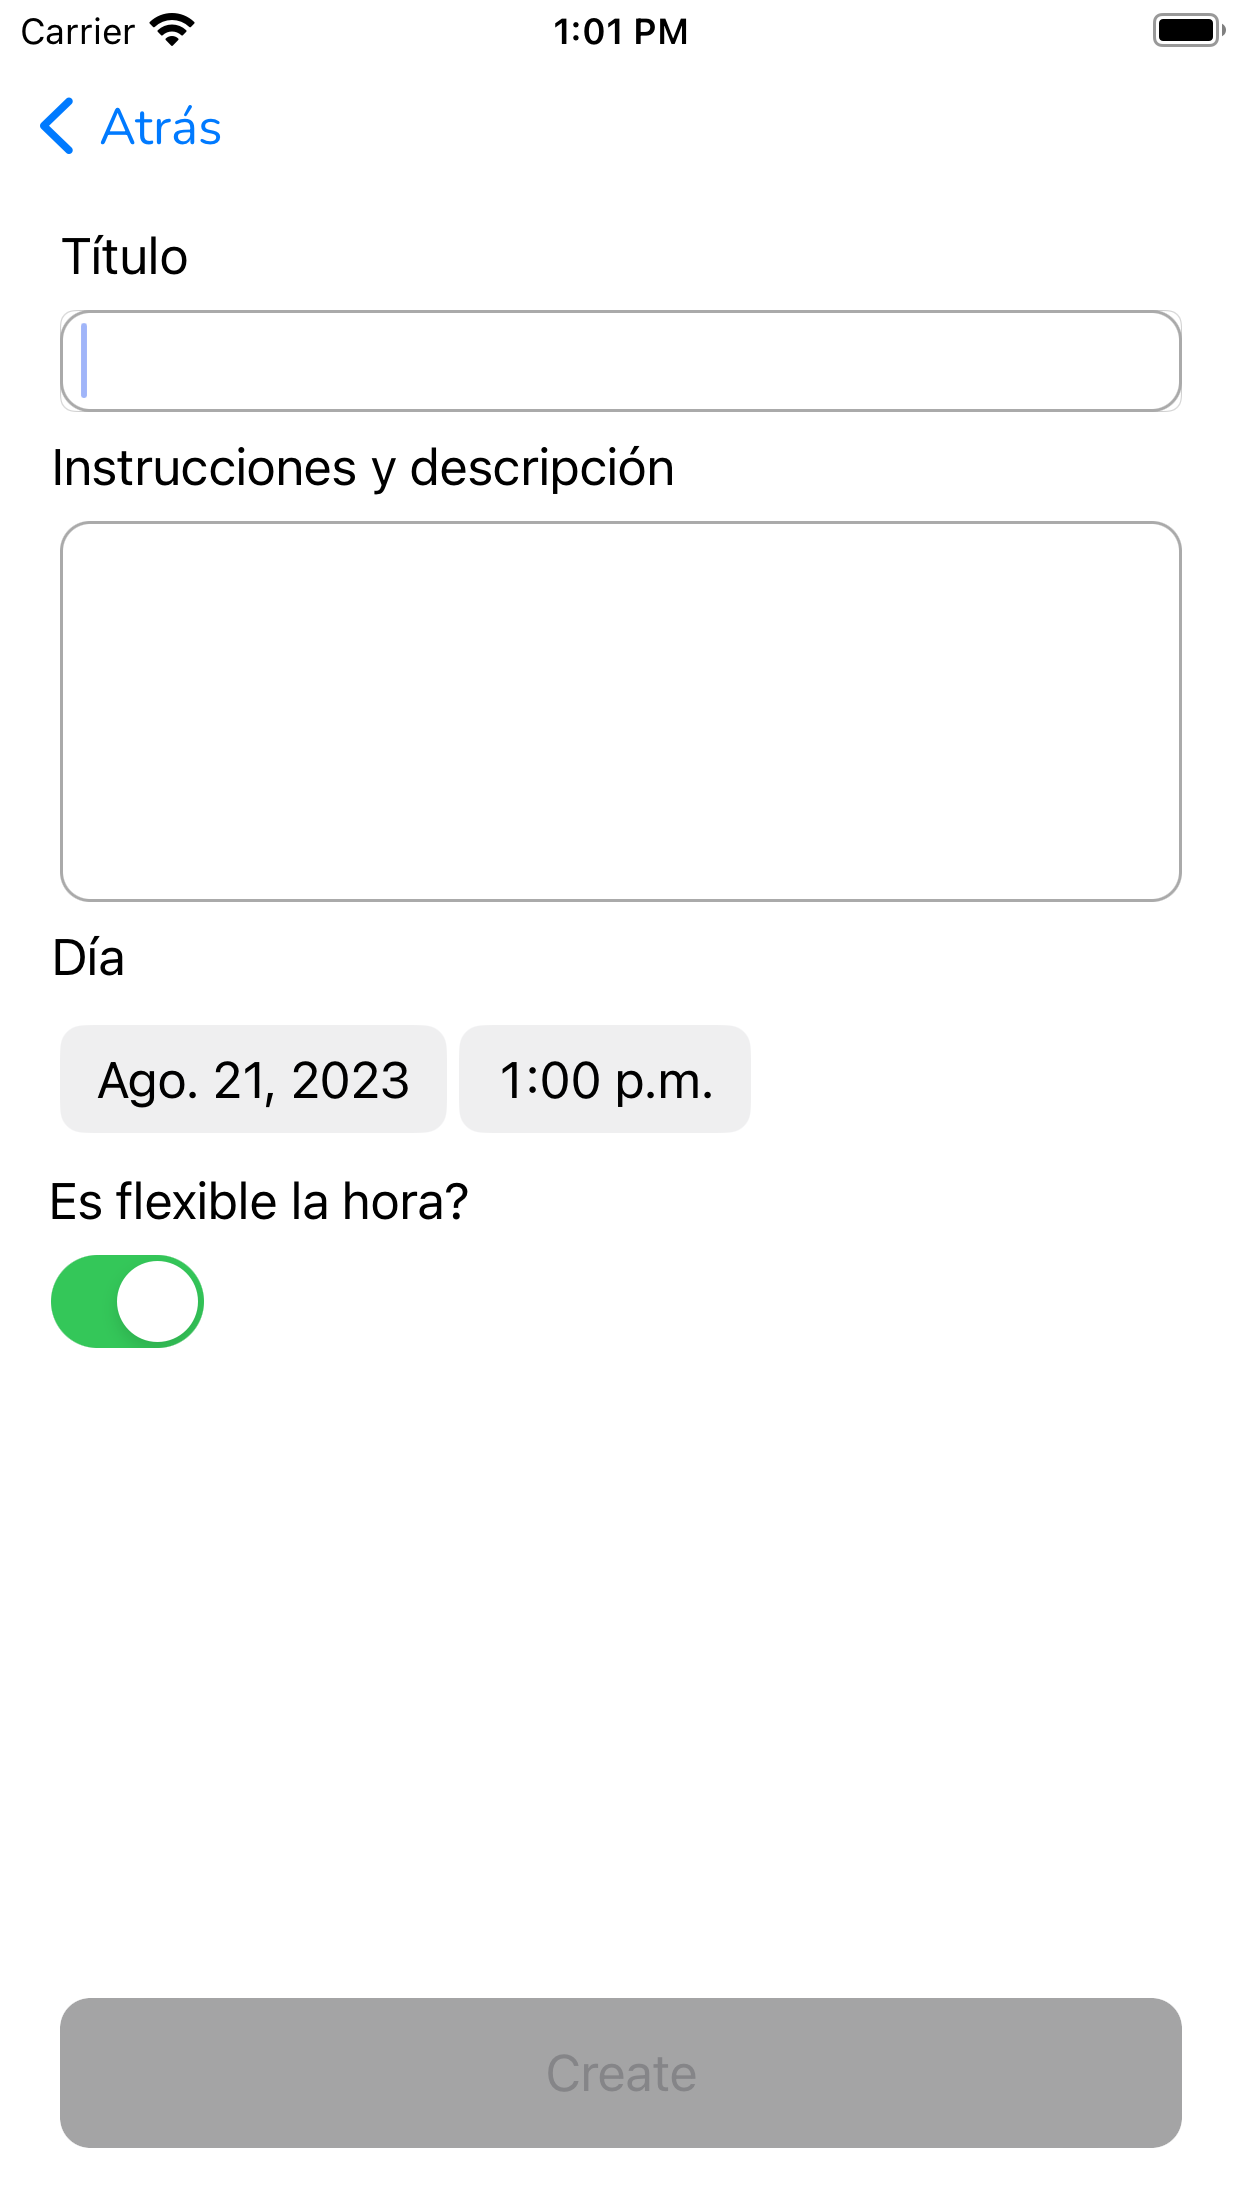
\includegraphics[cframe=black 2pt,width=0.3\linewidth]{images/manual/crearEventoFormulario.png}
        \caption{Vista creación de evento}
        \label{fig:Eventos}
\end{figure}
\begin{figure}[H]
        \centering
        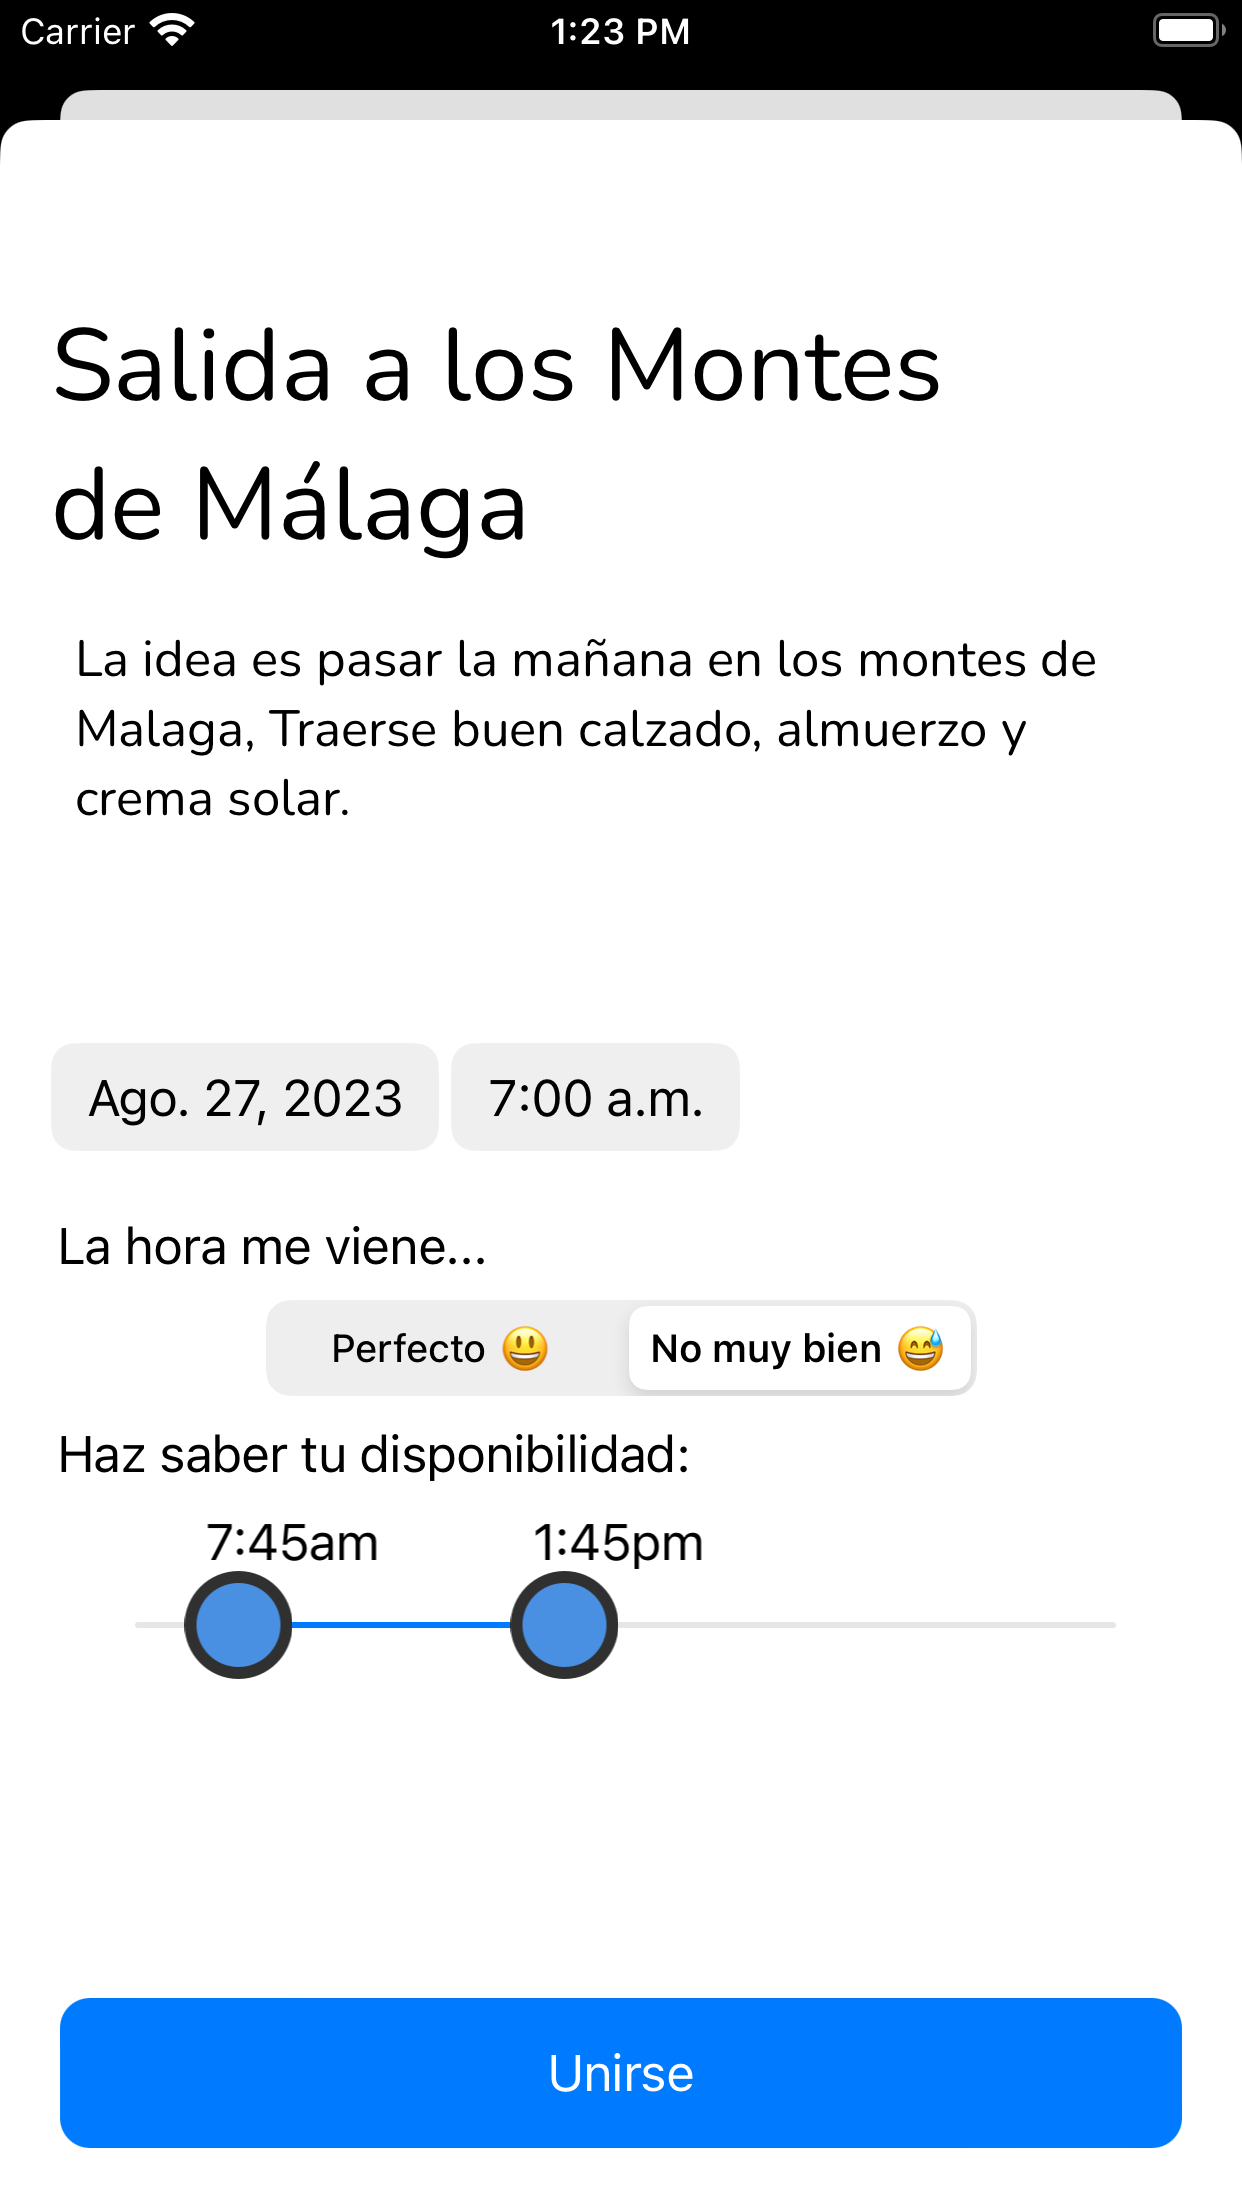
\includegraphics[cframe=black 2pt,width=0.3\linewidth]{images/manual/unirseAEvento.png}
        \caption{Vista apuntarse a evento}
        \label{fig:Vista unirse evento}
\end{figure}

\subsection{Estructura del proyecto}
\begin{figure}[H]
        \centering
        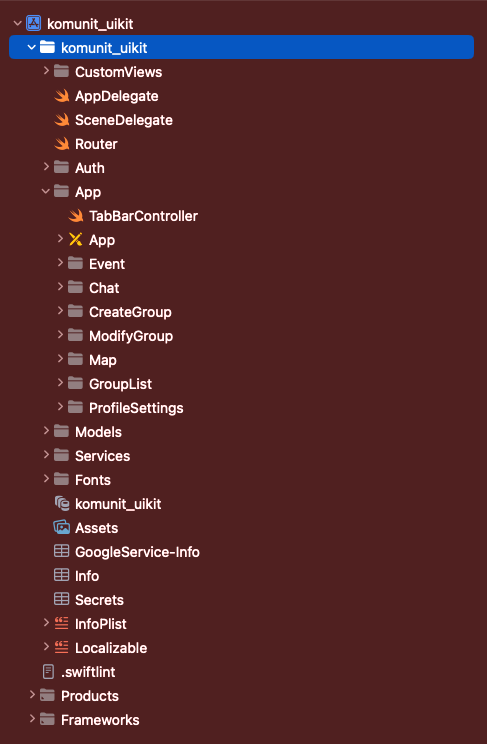
\includegraphics[width=0.66\linewidth]{images/manual/estructuraDelProyecto.png}
        \caption{Estructura del proyecto}
        \label{fig:estructuraProyecto}
\end{figure}
En la figura \ref{fig:estructuraProyecto} se puede observar la jerarquía del proyecto. A continuación, se detallan los directorios y archivos más relevantes que componen la estructura del proyecto:

\begin{enumerate}
        \item \textbf{AppDelegate.swift}: Es el archivo encargado de ser el punto de entrada de la aplicación. Configura Firebase, establece la apariencia de la aplicación y administra los eventos del ciclo de vida.
        \item \textbf{SceneDelegate.swift}: Esta clase es encargada de la gestión de las escenas de la aplicación, incluyendo la configuración del controlador de vista inicial conforme al estado de autenticación del usuario y la gestión de la alternancia entre los modos de visualización.
        \item \textbf{Router.swift}: La responsabilidad de esta clase radica en la administración de la navegación de la aplicación, determinando qué controlador de vista mostrar en función del estado de autenticación del usuario.
        \item \textbf{Auth}: Directorio que incluye las clases y recursos asociados con el proceso de autenticación de la aplicación, comprendiendo controladores de vista para el registro, la confirmación por correo electrónico, entre otros.
        \item \textbf{App}: Directorio que alberga las clases y recursos correspondientes a la parte principal de la aplicación, siendo el punto de interacción para los usuarios una vez iniciada la sesión.
        \item \textbf{Services}: Directorio que agrupa los servicios empleados en la aplicación, es decir, las clases que se encargan de la comunicación con la base de datos.
        \item \textbf{Models}: Directorio que contiene los modelos de datos empleados en la aplicación.
        \item \textbf{CustomViews}: Directorio en el cual se encuentran componentes de interfaz de usuario personalizados, utilizados en distintas partes de la aplicación.
        \item \textbf{Animations}: Directorio que alberga archivos de animación empleados en la aplicación.
        \item \textbf{Assets.xcassets}: Directorio que incluye los activos de imagen y color que se utilizan en la aplicación.
        \item \textbf{Fonts}: Directorio que contiene las fuentes tipográficas personalizadas que se emplean en la aplicación.
        \item \textbf{Localization}: La aplicación admite la localización, reflejada en la presencia de archivos de storyboard y archivos de cadena localizados, como es.lproj/Auth.strings y en.lproj/Localizable.strings.
        \item \textbf{komunit\_uikit.xcodeproj}: Archivo de proyecto de Xcode que reúne todas las configuraciones relacionadas con el proyecto.
\end{enumerate}






